\documentclass[../report.tex]{subfiles}
\begin{document}
\graphicspath{{img/}{../img/}}


\chapter{Proof of concept}

\blockquote{
We can only evaluate the user experience afforded by the toolkit and its features by building applications that use it, and then evaluating them. While the toolkit itself can be evaluated on its technical criteria, the aspects of it that are designed to support a particular user experience can only be evaluated in the context of use and thus must be evaluated indirectly - through applications built with the toolkit. \cite{Infrastructure (2003)} \\}

In previous chapters we evaluated Ocon on it's technical criteria by the design and choices made. In this chapter we will answer to our \textit{Goal 2} by implementing Ocon.

\section{Motivation}

Proof of concept will be a digital context-aware Scrumboard, and in this section we will briefly describe our motivation for this choice.

%Scrum is a popular agile process of developing software. Originally thought as using a whiteboard for scheduling development tasks, it has been hard for to make use of Scrum in distributed teams, or 



%Scrum is a popular agile process for developing software. In modern Scrum the task board is center of activity planning. It can be a whiteboard where tasks are coordinated, estimated and assigned. For more on Scrum see \textit{Scrum.org}.
%Center of focus is the whiteboard where tasks are coordinated, estimated and assigned. For more on Scrum see \textit{scrum.org}.

Scrum is a popular agile process for developing software. It focuses on rigid disciplines with timeboxing. Our motivation lies as part of the discipline of sprinting, and more precisely on the Scrumboard which has been adapted as a means to articulate the tasks in focus. This articulation is an important factor in teamwork which under the term articulation work describes the effort a team puts into communication.

The classic physique of the Scrumboard is a whiteboard with post-its, but two reasons have been the driving force behind development of digital Scrumboards.

\begin{itemize}
\item The whiteboard is analog, and there is labor in digitalizing it, for example for a Scrummaster to calculate burndowns or velocity.
\item Distributed Scrum teams have become more frequent with off-shoring and they need a digital solution for organizing tasks.
\end{itemize}

Many tools have sprung up motivated of these factors\footnote{Confluence, Scrumwise, Team Foundation, Trello}. These tools are not on par with the whiteboard when it comes to decreasing articulation work, because they lack the physical presence that the whiteboard has with a team. They do however solve the problems of distribution and digitalization.

\begin{itemize}
\item[\textbf{Motivation 1}] \textit{Popular digital Scrum tools are intended to be used by individuals. This increases articulation work}
\end{itemize}

Expanding on this is the motivation for context awareness as described in section \ref{sec:Context awareness} on page \pageref{sec:Context awareness}.

\begin{itemize}
\item[\textbf{Motivation 2}] \textit{Context awareness can improve the interaction between technology and humans}
\end{itemize}



Going forward in this chapter we will look to implement an idea of how these motivations could be satisfied by means of a digital Scrumboard and Ocon.


%We ourselves have used Scrum for several projects but never with the pleasure of a physical Scrumboard. We never had a room allocated and it simply wasn't possible to maintain a physical Scrumboard in a new space every day.


%A lot of tools for this problem have sprung up\footnote{Confluence, Scrumwise, Team Foundation, Trello} and made Scrum possible in this scenario, and even for a fully distributed team who would not be gathered physically in the first place.




%\begin{itemize}
%\item[] \Large{There is no solution today that digitalizes the whiteboard while maintaining it's presence}
%\end{itemize}

%\normalsize
%\vspace{0.2cm}

%This project does not cover implementation of a solution to these problems, but a some good ideas on it




\section{Context awareness}

The Scrumboard's purpose as a boundary object is to display information relevant to the team. The relevant information for the team depends on the situation, 
We have chosen three situations in Scrum where we believe the Scrumboard can benefit the team in having Context awareness

\begin{itemize}
\item Overview
\item Closeup
\item Standup
\end{itemize}

There are two situations we deem important which we want the Scrumboard to act upon:

\begin{itemize}
\item The standup meeting: When more than one person is standing in front of the Board
\item An individual closeup with the board
\end{itemize}

Actuation on these situations is purely graphical. There will be change in the graphical interface according to which information the interactors are interested in given the situation.

\begin{itemize}
\item Standup
\item Closeup
\item Overview. This view is our default for when none of the other contexts are true
\end{itemize}


\todo{more explanation of the context involved and how we'll represent it with OCon...}



\section{Implementation and environment}

The Context-aware Scrumboard consists of three parts: The KinectEntitySensor, The Centralization and the Scrumboard. These parts are distributed and communicate with the OconTcpCom implementation over LAN from each of their own hardware nodes.

\begin{figure}[H]
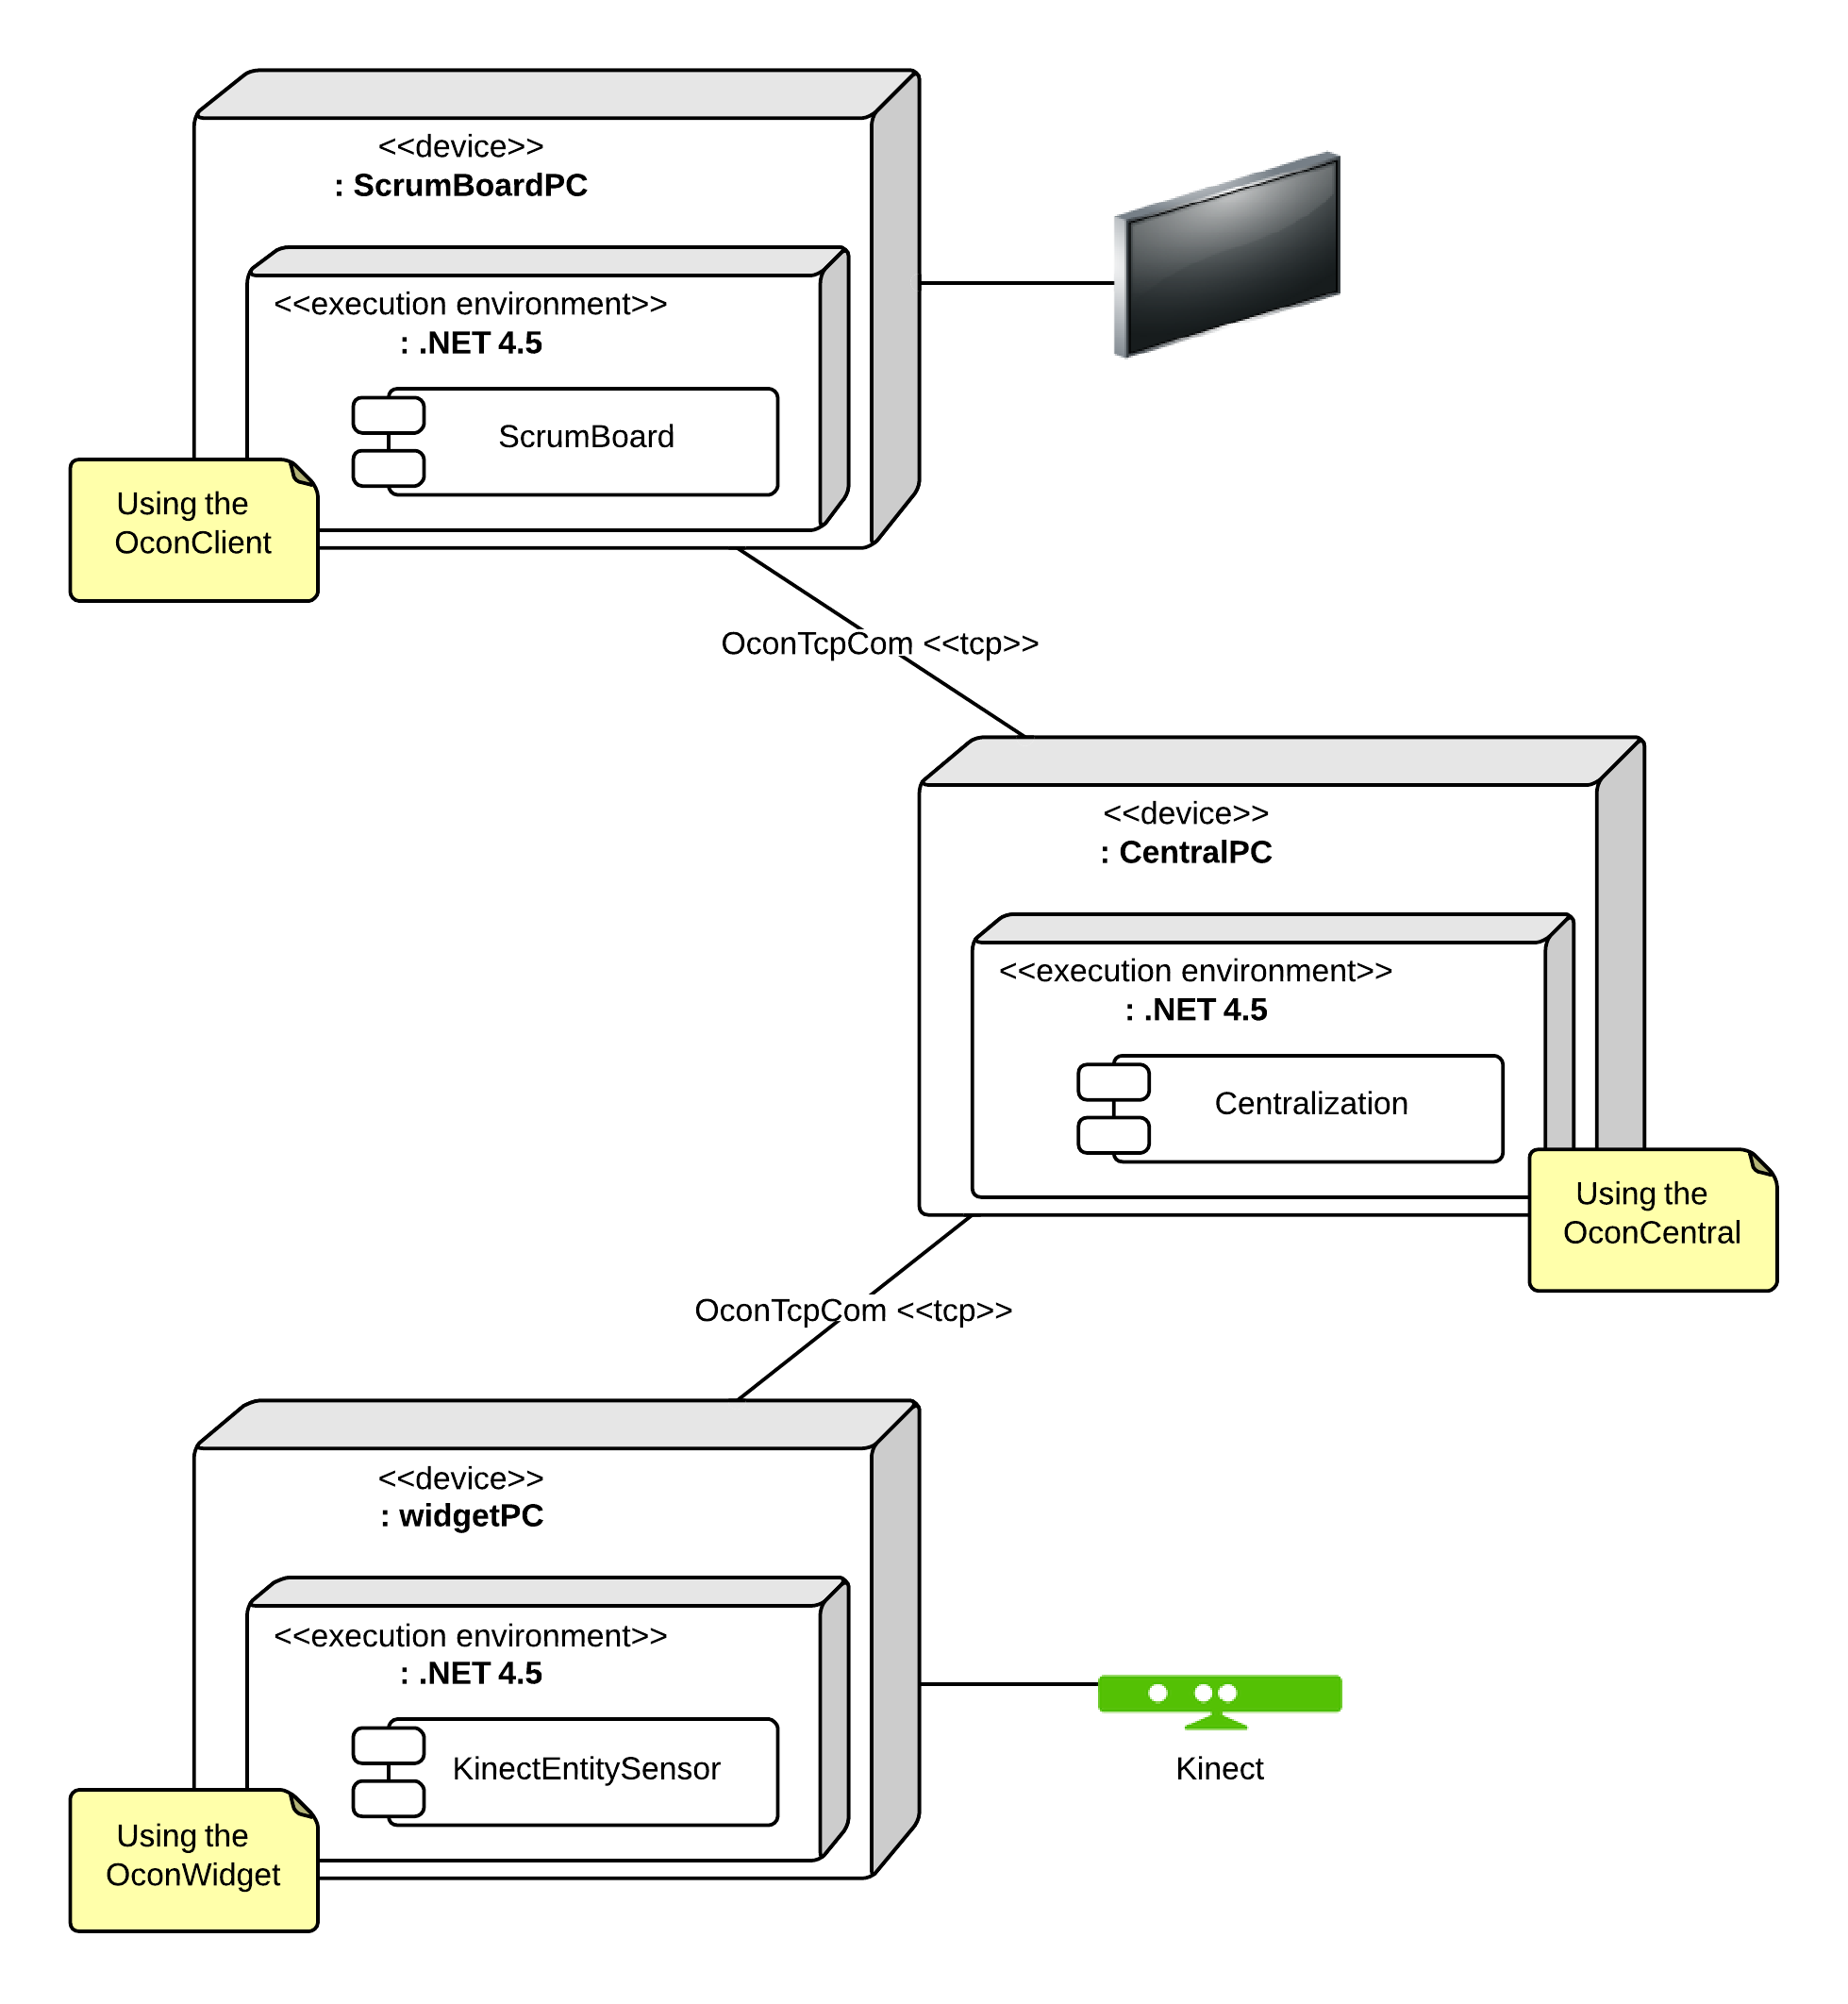
\includegraphics[width=\linewidth]{./ProofOfConceptDeployment.png}
\caption{Proof of concept deployment}
\label{fig:ProofofConceptDeployment}
\end{figure}

\subsection{The KinectEntitySensor}
The KinectEntitySensor's task is to gather Context Information and send it to the centralization. Ocon has been implemented to help with that. This part of the Context-aware Scrumboard implementation involves transferring information to the OconCentral, and it is for that purpose the OconWidget has been implemented.

The widget's task is to translate sensor data into IEntity implementation types and pass them to the OconWidget which will handle transfering it to the central.
\begin{figure}[H]
\begin{lstlisting}
//Instantiate a logging instance
var log = Console.Out;
//for file logging: new StreamWriter("/file/path/here");

//Instantiate an IOconCom implementation
var com = new OconTcpCom(log);

//Instantiate widget
var widget = new OconWidget(com, log);

//Start searching for a central with the given IOconCom implementation
widget.StartDiscovery();

//Pass an entity to be added/updated at the central
var entity = new Person() { Name = "Mat", Present = true };
widget.Notify(entity);
\end{lstlisting}
\caption{Widget usage from TestWidget.Program}
\label{code:OconWidget}
\end{figure}



\subsection{The centralization}
The central
\begin{figure}[H]
\begin{lstlisting}
//Instantiate a logging instance
var log = Console.Out;

//Instantiate an IOconCom implementation
var tcpCom = new OconTcpCom(log);

//Instantiate the context filter
var oconFilter = new OconContextFilter(log);

//Instantiate situations with names and predicates
var closeupSituation = new Situation("Closeup", e => e.OfType<Person>().Count(p => p.Present) == 1);
var standupSituation = new Situation("Standup", e => e.OfType<Person>().Count(p => p.Present) == 2);

//Add the situations to the filter
oconFilter.AddSituation(closeupSituation, standupSituation);

//Instantiate the central
var central = new OconCentral(oconFilter, tcpCom, log);

//Initialize the central
central.Initialize();
\end{lstlisting}
\caption{Central usage from TestCentral.Program}
\label{code:OconCentral}
\end{figure}

\subsection{The Scrumboard}

\begin{figure}[H]
\begin{lstlisting}
//Choose a logging instance if any
var log = Console.Out;

//Instantiate a network helper. Here passing the logging target
//alternatively instantiate as new TcpHelper(); if no logging is needed
var comHelper = new OconTcpCom(log);

//Instantiate the client with communication, log, and params of situation names strings
var oconClient = new OconClient(comHelper, log, StandupSituationString, CloseupSituationString);

//Subscribe a delegate to be run when a situation change event is fired
oconClient.SituationStateChangedEvent += (sender, args) => UpdatePicture(args.SituationName, args.State);
\end{lstlisting}
\caption{Client usage from OconScrumBoard.MainViewModel}
\label{code:OconClient}
\end{figure}


\todo{This solution with the elements from blackboard makes development very uncoupled. The blackboard requires a consensus and so Widget/sensor and client can be implemented independently}


\end{document}